\documentclass[border=4pt,12pt]{standalone}
% House style for redrawn exam diagrams (diagram-v4: 0.4pt lines, filled -latex arrows, fine dashes; stipple and hatching drawn as real dots/lines (no PDF/SVG patterns, so they render in every browser and at any scale); transparent background). Every figure \input's this.
\usepackage{amsmath,amssymb}
\usepackage{txfonts}
\usepackage{pdfrender,xcolor}
% \halo{text}: label on shading. The shading stops just around each letter's outline (a thin knock-out that follows the
% glyphs, like the papers' typesetting), never a box. Owner: "I don't want a box around the text".
\newcommand{\halo}[1]{\leavevmode\rlap{\pdfrender{TextRenderingMode=2,LineWidth=2.2pt,LineJoinStyle=1,StrokeColor=white,FillColor=white}#1}#1}
\usepackage{tikz,pgfplots}
\pgfplotsset{compat=1.18}
\usetikzlibrary{arrows.meta,calc,angles,quotes,patterns,patterns.meta,intersections,positioning,decorations.markings,shapes.geometric}
% Stipple and hatching are drawn as actual dots / lines clipped to the region (path picture), NOT as pattern fills:
% SVG <pattern> fills vanish or blur when browsers scale the image, so the owner could not see the shading.
% Each dot is a 0.72pt square (keeps SVGs small; reads as a dot at print size). Dots sit on one global staggered grid, so neighbouring regions line up.
\makeatletter
\newdimen\ex@x \newdimen\ex@y \newdimen\ex@xa \newdimen\ex@ya \newdimen\ex@xb \newdimen\ex@yb \newcount\ex@row
\def\exam@stipplecolor{black!75}\def\exam@dotr{0.42pt}\def\exam@dotgap{2.5}
\def\ex@rowdots{\ifdim\ex@x<\ex@xb \pgfpathrectangle{\pgfqpoint{\dimexpr\ex@x-0.36pt\relax}{\dimexpr\ex@y-0.36pt\relax}}{\pgfqpoint{0.72pt}{0.72pt}}\advance\ex@x by \exam@dotgap pt\relax\expandafter\ex@rowdots\fi}
\def\exam@stipple{%
  \pgftransformreset% dots are sized in real points even inside scaled pictures
  \pgfpointanchor{path picture bounding box}{south west}\ex@xa=\pgf@x \ex@ya=\pgf@y
  \pgfpointanchor{path picture bounding box}{north east}\ex@xb=\pgf@x \ex@yb=\pgf@y
  \pgfsetfillcolor{\exam@stipplecolor}\pgfmathsetmacro\ex@h{\exam@dotgap/2}%
  \pgfmathtruncatemacro\ex@r{floor(\ex@ya/\ex@h)-1}\ex@row=\ex@r\relax
  \ex@y=\ex@r\dimexpr\ex@h pt\relax
  \loop\ifdim\ex@y<\ex@yb
    \pgfmathtruncatemacro\ex@c{floor(\ex@xa/\exam@dotgap)-1}\ex@x=\ex@c\dimexpr\exam@dotgap pt\relax
    \ifodd\ex@row \advance\ex@x by \ex@h pt\fi
    \ex@rowdots
    \advance\ex@y by \ex@h pt \advance\ex@row by 1
    \ifnum\numexpr\ex@row-(\ex@row/4)*4\relax=0 \pgfusepath{fill}\fi% flush every 4 rows: bounded TeX memory, few clip copies in the SVG
  \repeat\pgfusepath{fill}}
\newdimen\ex@d
\def\exam@hatch#1{% #1 = 1 for /, -1 for \ ; lines 45 degrees, 3pt apart
  \pgftransformreset
  \pgfpointanchor{path picture bounding box}{south west}\ex@xa=\pgf@x \ex@ya=\pgf@y
  \pgfpointanchor{path picture bounding box}{north east}\ex@xb=\pgf@x \ex@yb=\pgf@y
  \ex@d=\dimexpr\ex@yb-\ex@ya\relax \ex@x=\dimexpr\ex@xa-\ex@d\relax
  \loop\ifdim\ex@x<\ex@xb
    \ifnum#1>0 \pgfpathmoveto{\pgfqpoint{\ex@x}{\ex@ya}}\pgfpathlineto{\pgfqpoint{\dimexpr\ex@x+\ex@d\relax}{\ex@yb}}%
    \else \pgfpathmoveto{\pgfqpoint{\ex@x}{\ex@yb}}\pgfpathlineto{\pgfqpoint{\dimexpr\ex@x+\ex@d\relax}{\ex@ya}}\fi
    \advance\ex@x by 4.24pt
  \repeat
  \pgfsetlinewidth{0.4pt}\pgfsetstrokecolor{black}\pgfusepath{stroke}}
\def\examstipple{\exam@stipple}\def\examhatch{\exam@hatch}\def\examsetstipplecolor#1{\def\exam@stipplecolor{#1}}\def\examsetdotgap#1{\def\exam@dotgap{#1}}
\makeatother
% (legacy pattern kept for old files)
% staggered stipple like the NESA papers' dotted shading
\pgfdeclarepatternformonly{exam stipple}{\pgfpointorigin}{\pgfqpoint{2.2pt}{2.2pt}}{\pgfqpoint{2.2pt}{2.2pt}}{%
  \pgfpathcircle{\pgfqpoint{0.55pt}{0.55pt}}{0.42pt}\pgfpathcircle{\pgfqpoint{1.65pt}{1.65pt}}{0.42pt}\pgfusepath{fill}}
\tikzset{
  every picture/.style={line width=0.6pt, >={Latex[length=2mm,width=1.3mm]}},
  curve/.style={line width=0.6pt},
  open arrow/.style={-{Latex[length=2mm,width=1.3mm]}},  % owner: filled -latex heads everywhere, no open chevrons
  aux/.style={dash pattern=on 2pt off 1.5pt, line width=0.6pt},
  shade/.code={\def\exA{#1}\def\exB{none}\ifx\exA\exB\else\pgfkeysalso{fill=black!18}\fi},
  shade/.default=on,
  shade dots/.style={fill=none, path picture={\examstipple}},
  stipple color/.code={\examsetstipplecolor{#1}},
  stipple gap/.code={\examsetdotgap{#1}},
  shade dense dots/.style={fill=none, stipple gap=1.6, path picture={\examstipple}},
  shade hatch/.style={fill=none, path picture={\examhatch{1}}},
  shade hatch reverse/.style={fill=none, path picture={\examhatch{-1}}},
  shade solid/.style={fill=black},
  pt/.style={circle, fill, inner sep=1.1pt},
  open pt/.style={circle, draw, fill=white, inner sep=1.1pt},
}
\pgfplotsset{
  exam axes/.style={axis lines=middle, axis line style={->}, xlabel={$x$}, ylabel={$y$},
    xlabel style={anchor=west}, ylabel style={anchor=south}, tick label style={font=\small},
    every axis plot/.append style={line width=0.6pt, black}, samples=200, clip=false,
    enlargelimits=false, axis on top},
}

\begin{document}
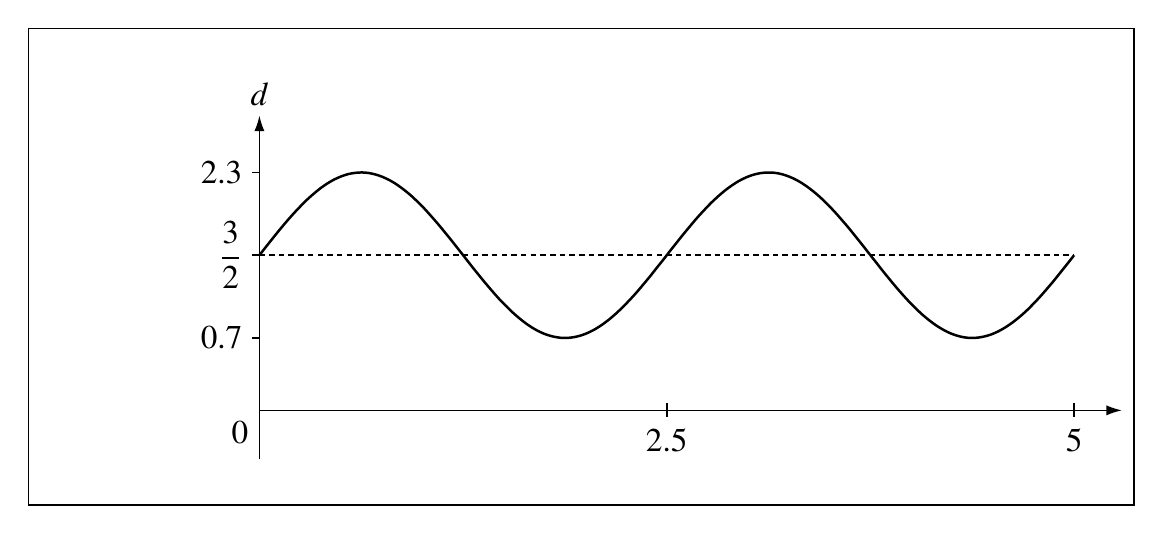
\begin{tikzpicture}[x=0.0127cm, y=-0.0127cm]
\draw (1,1) rectangle (1107,478);
\draw[->] (232,383) -- (1095,383);
\draw[->] (232,432) -- (232,88);
\draw[aux] (232,227.8) -- (1047.0,227.8);
\draw[line width=0.9pt] plot[smooth] coordinates {(232.0,227.8) (238.8,219.1) (245.7,210.4) (252.5,202.0) (259.4,193.8) (266.2,186.1) (273.1,178.8) (279.9,172.0) (286.8,165.9) (293.6,160.4) (300.5,155.7) (307.3,151.8) (314.2,148.8) (321.0,146.6) (327.9,145.4) (334.7,145.0) (341.6,145.6) (348.4,147.1) (355.3,149.5) (362.1,152.7) (369.0,156.8) (375.8,161.7) (382.7,167.3) (389.5,173.6) (396.4,180.5) (403.2,188.0) (410.1,195.9) (416.9,204.1) (423.8,212.6) (430.6,221.2) (437.5,230.0) (444.3,238.7) (451.2,247.3) (458.0,255.6) (464.9,263.7) (471.7,271.4) (478.6,278.5) (485.4,285.1) (492.3,291.1) (499.1,296.4) (505.9,300.9) (512.8,304.6) (519.6,307.4) (526.5,309.3) (533.3,310.4) (540.2,310.5) (547.0,309.7) (553.9,308.0) (560.7,305.4) (567.6,301.9) (574.4,297.6) (581.3,292.5) (588.1,286.7) (595.0,280.2) (601.8,273.2) (608.7,265.7) (615.5,257.7) (622.4,249.4) (629.2,240.8) (636.1,232.2) (642.9,223.4) (649.8,214.7) (656.6,206.2) (663.5,197.9) (670.3,189.9) (677.2,182.4) (684.0,175.3) (690.9,168.9) (697.7,163.1) (704.6,158.0) (711.4,153.7) (718.3,150.2) (725.1,147.6) (732.0,145.9) (738.8,145.1) (745.7,145.2) (752.5,146.2) (759.4,148.2) (766.2,151.0) (773.1,154.7) (779.9,159.2) (786.7,164.4) (793.6,170.4) (800.4,177.0) (807.3,184.2) (814.1,191.9) (821.0,199.9) (827.8,208.3) (834.7,216.9) (841.5,225.6) (848.4,234.3) (855.2,243.0) (862.1,251.5) (868.9,259.7) (875.8,267.6) (882.6,275.0) (889.5,281.9) (896.3,288.2) (903.2,293.8) (910.0,298.7) (916.9,302.8) (923.7,306.1) (930.6,308.5) (937.4,310.0) (944.3,310.6) (951.1,310.2) (958.0,308.9) (964.8,306.8) (971.7,303.7) (978.5,299.8) (985.4,295.1) (992.2,289.7) (999.1,283.6) (1005.9,276.8) (1012.8,269.5) (1019.6,261.7) (1026.5,253.6) (1033.3,245.1) (1040.2,236.5) (1047.0,227.8)};
\foreach \v in {0.7,2.3} \draw (225,{383-103.478*\v}) -- (232,{383-103.478*\v});
\draw (225,227.8) -- (232,227.8);
\foreach \t in {2.5,5} \draw ({232+163.000*\t},376) -- ({232+163.000*\t},390);
\node[font=\large, anchor=east, inner sep=3pt] at (224,145.0) {$2.3$};
\node[font=\large, anchor=east, inner sep=3pt] at (224,310.6) {$0.7$};
\node[font=\large, anchor=east, inner sep=3pt] at (224,227.8) {$\dfrac{3}{2}$};
\node[font=\large, anchor=north east, inner sep=3pt] at (230,385) {$0$};
\node[font=\large, anchor=north, inner sep=5pt] at (639.5,387) {$2.5$};
\node[font=\large, anchor=north, inner sep=5pt] at (1047.0,387) {$5$};
\node[font=\large, anchor=south, inner sep=3pt] at (232,88) {$d$};
\end{tikzpicture}
\end{document}
